\documentclass[11pt,a4paper]{article}

\usepackage[T1]{fontenc}
\usepackage[utf8]{inputenc}
\usepackage[margin=2.4cm]{geometry}
\usepackage{graphicx}
\usepackage{amsmath,amssymb}
\usepackage{bm}
\usepackage{hyperref}
\usepackage{xcolor}
\usepackage{siunitx}
\usepackage{booktabs}
\usepackage{natbib}
\usepackage{caption}
% Cross-reference the main manuscript (e.g. Eq.~(b)); needs
% manuscript.aux, so compile the main file first (the Makefile does).
\usepackage{xr-hyper}
\externaldocument{manuscript}

\captionsetup{font=small,labelfont=bf,labelsep=period,justification=raggedright,singlelinecheck=false}

\hypersetup{colorlinks=true, linkcolor=blue!50!black, citecolor=blue!50!black, urlcolor=blue!50!black}

\graphicspath{{figures/}}

% S-numbering for supplementary figures and tables.
\renewcommand{\thefigure}{S\arabic{figure}}
\renewcommand{\thetable}{S\arabic{table}}
\renewcommand{\theequation}{S\arabic{equation}}

\begin{document}

\title{Supplementary Material\\[0.4em]
\large Density-gated noise rectification in a Vicsek--Couzin
flock: one dense-phase mechanism, additive at matched
decorrelation}

\author{Yaya Youssouf Yaya \quad Mamadou Sy}

\date{\today}

\maketitle

\subsection*{Order-parameter distribution at $L = 30$}

The Binder dip is ambiguous on its own: a weakly first-order
transition deepens $U_4$ through a bimodal
$P(\langle\varphi\rangle)$, while a continuous transition with
large $\gamma/\nu$ deepens it without bimodality. Only the
full distribution separates the two. We histogram
$\langle\varphi\rangle$ on long trajectories at $L = 30$,
$N = 2000$, three seeds, $6000$ measurement steps each, for
the motility-only ablation at $\eta = 0.10$ and the
double-adaptive model at $\eta = 0.15$
(Fig.~\ref{fig:transition}a). Both histograms come out unimodal.

\begin{figure}[htbp]
    \centering
    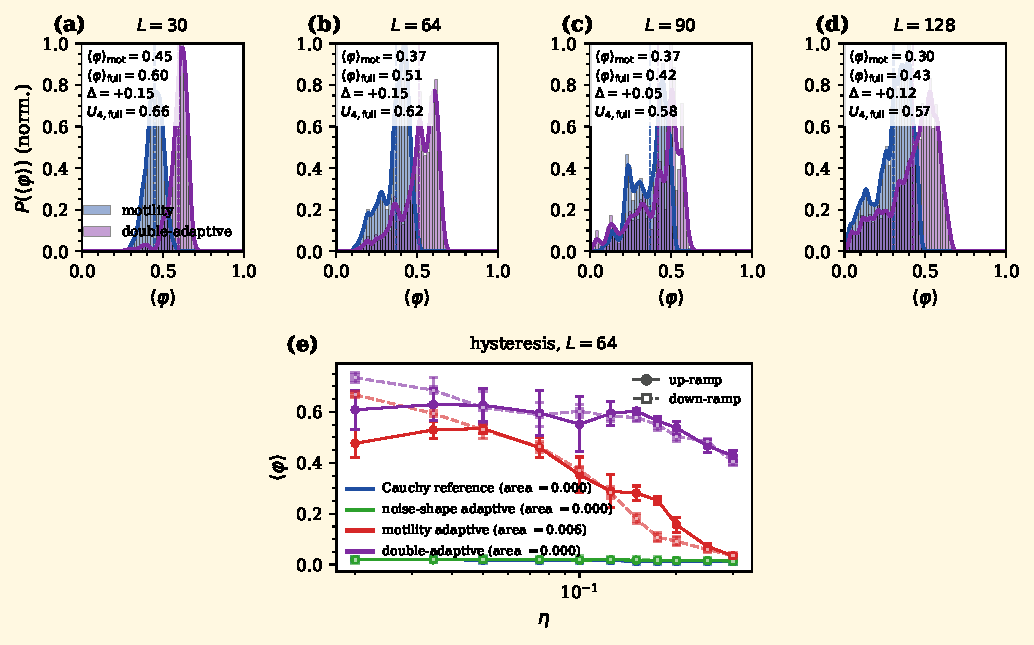
\includegraphics[width=\linewidth]{fig_double_transition.pdf}
    \caption{Order of the transition. (a)--(d)
    order-parameter distribution $P(\langle\varphi\rangle)$ with
    motility-only and double-adaptive overlaid, one panel per size
    (a) $L = 30$, (b) $L = 64$, (c) $L = 90$, (d) $L = 128$ (motility
    at $\eta = 0.10$, double-adaptive at $\eta = 0.15$), each
    normalised to its own peak and sharing the vertical scale; dashed
    lines mark the per-mode means and each panel reports the mean gap
    $\Delta$ and the full-mode Binder cumulant $U_4$. (e)
    quasi-static $\eta$ ramp up (filled circles, solid) and down
    (open squares, dashed) at $L = 64$, five seeds, the two
    motility-active modes (hue), with the loop areas. $P(\langle\varphi\rangle)$ stays
    single-peaked at every size and the hysteresis loops are
    negligible ($\leq 0.006$): the deepened Binder dip is not a
    coexistence signature and the transition is continuous (at most
    very weakly first-order).}
    \label{fig:transition}
\end{figure}

Motility-only peaks at $\langle\varphi\rangle \simeq 0.45$
with skewness $-0.25$, kurtosis $-0.14$ (a mildly left-skewed
broad mode); the double-adaptive model peaks at $0.60$ with
a sharper core (kurtosis $+5.56$) and a long left tail
(skewness $-1.88$). The long-trajectory Binder cumulants
$U_4 = 0.65$ (motility) and $0.66$ (full) sit just below the
bimodal limit $U_4 \to 2/3$ and well above the Gaussian
$U_4 = 0$: the trajectories are locked in a single ordered
state with bounded fluctuations, not switching between two
phases. The transition is at most weakly first-order here.

Rerunning the histograms at $L = 64, 90$ (five seeds,
$6\,000$ steps) and at $L = 128$ (five seeds, $60\,000$
steps) in panels (b)--(d), the double-adaptive distribution
sits to the right of motility-only at every size:
$\Delta\langle\varphi\rangle = +0.145, +0.048, +0.121$ at
$L = 64, 90, 128$ (the $L = 90$ row a seed-budget outlier
already seen in $s_{\rm sep}$). The full-mode $U_4$ stays in
$[0.57, 0.62]$ and the distributions broaden into mildly
platykurtic shapes at $L = 128$ ($\kappa = -0.27$ for
motility, $-0.20$ for full) without developing two-peak
structure. $P(\langle\varphi\rangle)$ remains unimodal across
all four sizes.

\subsection*{Hysteresis across the transition}
\label{sec:hysteresis}

The unimodal $P(\langle\varphi\rangle)$ and the ambiguous
$U_4$ dip leave the order of the transition unsettled; a
hysteresis test settles it. We ramp $\eta$ quasi-statically
up and back down at $L = 64$, five seeds, carrying the
configuration over from one step to the next (no
re-randomisation), for the two motility-active modes
(Fig.~\ref{fig:transition}e). The up- and down-ramp
$\varphi(\eta)$ branches overlap within error bars and the
loop area is negligible: $0.006$ for motility-only,
$0.000$ for the double-adaptive model. A first-order
transition would open a finite loop; its absence, with the
unimodal $P(\langle\varphi\rangle)$, places the transition in
the continuous (or at most very weakly first-order) class.

\subsection*{Time-averaged density profile along the polar axis}

The dense phase still has to be characterised geometrically:
does it travel as a metric-Vicsek soliton or sit as an
isotropic patch comoving with the flow? The band-soliton
index $b$ of Eq.~\eqref{eq:b} discriminates
($b \gtrsim 1.5$ for a band, $b \simeq 1$ for a patch). We
measure $b$ for all four heavy-tailed modes at their
near-critical $\eta$, $L = 30$, three seeds, $4000$
measurement steps (Fig.~\ref{fig:profile}).

\begin{figure}[htbp]
    \centering
    
\includegraphics[width=0.95\linewidth]{fig_double_profile.pdf}
    \caption{Time-averaged profiles along the instantaneous
    polar-flow axis $x_\parallel$ at $L = 30$, three seeds,
    $4000$ measurement steps, the four modes overlaid at
    their respective near-critical $\eta$. (a) density
    normalised to its peak, with the band-soliton index $b$ per
    mode in the legend. (b) local speed normalised to its
    peak. Every profile is flat ($b \simeq 1$), so the
    motility-built dense phase is an isotropic comoving patch, not a
    travelling Vicsek band.}
    \label{fig:profile}
\end{figure}

All four profiles are flat to within $7\,\%$ ($b = 1.01,
1.02, 1.04, 1.06$ in the order Cauchy, noise-shape, motility,
full). None supports a metric-Vicsek band: the motility-built
dense phase either reorganises faster
than its polar axis or is isotropic in the comoving frame.
The full mode is marginally the most cohesive, consistent
with the Gaussian rectification tightening the patch from
within, but the increment is well below the soliton
threshold.

\subsection*{Why $\chi_{\max}(L)$ is a crossover, not an exponent}

The log--log slopes $a_{\rm motility} = +1.04$ and
$a_{\rm full} = +1.49$ of Table~\ref{tab:slopes} (steeper still,
$+1.29$ and $+1.95$, on the seven-size sub-grid) are large enough
to invite a critical reading, so we test that reading directly
on the homogeneous ten-seed series
(Fig.~\ref{fig:collapse}). A genuine power law would hold a
\emph{constant} local slope $a_{\rm eff} = d\ln\chi_{\max}/
d\ln L$ across the range; instead, for both motility-active
modes $a_{\rm eff}$ overshoots its own global fit at
intermediate sizes and then falls back toward zero in the
largest interval ($L = 90 \to 128$ gives $a_{\rm eff} = +0.07$
for the full mode and $+0.13$ for motility-only), while the two
fixed-motility references stay pinned at $a_{\rm eff} \simeq 0$
(panel a). The growth is therefore a finite-size transient that
is already saturating at the top of our window, not a clean
asymptotic scaling.

\begin{figure}[htbp]
    \centering
    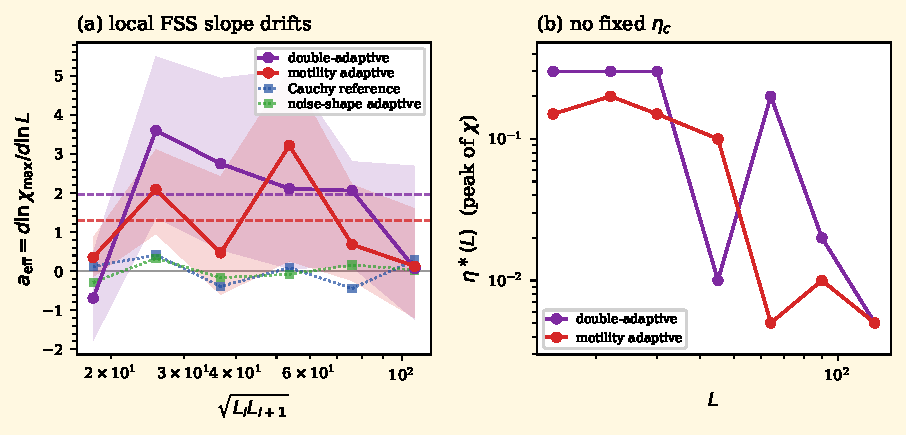
\includegraphics[width=\linewidth]{fig_double_collapse.pdf}
    \caption{Finite-size-scaling diagnostic on the homogeneous
    ten-seed series. (a) local effective slope
    $a_{\rm eff} = d\ln\chi_{\max}/d\ln L$ between consecutive
    sizes, plotted at the geometric-mean size; dashed lines mark
    each mode's global log--log fit. The two motility-active
    modes overshoot their global slope at intermediate $L$ and
    collapse toward zero in the largest interval, whereas the
    Cauchy and noise-shape references hug $a_{\rm eff}\simeq0$
    throughout; bands are $95\%$ seed bootstraps ($B=4000$). (b)
    position $\eta^\ast(L)$ of the susceptibility peak: instead of
    converging to a size-independent $\eta_c$, it migrates toward
    the small-$\eta$ boundary, so the scaling variable
    $(\eta-\eta_c)L^{1/\nu}$ of a standard collapse cannot be
    defined here.}
    \label{fig:collapse}
\end{figure}

A standard collapse $\chi/L^{a}$ against
$(\eta-\eta_c)L^{1/\nu}$ needs a size-independent critical point
$\eta_c$. Panel (b) shows there is none: the susceptibility peak
$\eta^\ast(L)$ does not settle but drifts toward the smallest
accessible noise as $L$ grows, the signature of an
order-from-density (MIPS-like) growth in which $\chi$ keeps
rising as $\eta \to 0$ rather than diverging at a finite
$\eta_c$. With the slope still drifting and the peak still
migrating, we report $a_{\rm full}$ and
$a_{\rm motility}$ as the growth rate of a finite-size
phase-separation susceptibility, and the each-own-$\eta$ excess
($\Delta_7 = +0.63$ on the seven-size sub-grid, $\Delta_9 = +0.45$
across all nine sizes) as a finite-size crossover gap rather than
a difference of asymptotic exponents. The matched-noise control
of the main text shows even this excess is a dense-noise effect:
retuning motility-only to the full mode's dense decorrelation
collapses it to $\Delta_9 = +0.02$.

\subsection*{Finite-size scaling at three global densities}
\label{sec:supp-density}

Is the two-regime split of the main text a property of the
motility channel, or of the working density $\rho_0 = 2.22$? We
answer it by repeating the finite-size scan at
$\rho_0 = 1.0$ and $3.0$ over the size range $22$ to $128$ common
to all three densities.

\begin{table}[h]
\centering
\caption{FSS slopes $a$ ($\chi_{\max} \sim L^a$, common sizes
$22$ to $128$, ten seeds, $95\%$ bootstrap CI) at three global
densities. The motility-active modes grow at every density while
the fixed-noise modes stay flat, and the noise-shape excess
$a_{\rm full} - a_{\rm motility}$ widens with $\rho_0$. The
$\rho_0 = 3.0$ value $+3.00$ exceeds the $d = 2$ ceiling
$\chi_{\max} \le N$, marking these as finite-size crossover rates,
not asymptotic exponents.}
\label{tab:density}
\small
\begin{tabular}{l c c c}
\toprule
Mode & $\rho_0 = 1.0$ & $\rho_0 = 2.22$ & $\rho_0 = 3.0$ \\
\midrule
fixed-noise ($\max|a|$) & $0.06$ & $0.09$ & $0.03$ \\
motility adaptive & $+0.64$ & $+1.37$ & $+2.00$ \\
                  & {\scriptsize $[+0.35,+0.84]$} & {\scriptsize $[+1.14,+2.02]$} & {\scriptsize $[+1.87,+2.22]$} \\
double-adaptive   & $+0.63$ & $+2.17$ & $+3.00$ \\
                  & {\scriptsize $[+0.32,+0.94]$} & {\scriptsize $[+1.88,+2.70]$} & {\scriptsize $[+2.74,+3.38]$} \\
\midrule
excess $a_{\rm full}-a_{\rm motility}$ & $-0.01$ & $+0.80$ & $+1.00$ \\
\bottomrule
\end{tabular}
\end{table}

Both motility-active modes grow at every density while the three
fixed-noise modes stay flat, and the noise-shape excess tracks
density: the full and motility-only slopes coincide at
$\rho_0 = 1.0$ ($+0.63$ against $+0.64$), separate by $\simeq +0.8$
at $\rho_0 = 2.22$ and by $+1.0$ at $\rho_0 = 3.0$ ($+3.00$ against
$+2.00$). These common-range slopes run steeper than the nine-size
values of Table~\ref{tab:slopes} ($a_{\rm full} = +1.49$ at
$\rho_0 = 2.22$) because they omit the two saturating sizes
$L = 180, 256$. That difference, together with the
$\rho_0 = 3.0$ value $+3.00$ exceeding the $d = 2$ ceiling
$\chi_{\max} \le N$, marks these slopes once more as finite-size
crossover rates and not asymptotic exponents. The density trend is
accordingly to be read qualitatively: an excess that grows with
$\rho_0$.

\subsection*{\texorpdfstring{Behavioural plane in $(n_\star, s)$}{Behavioural plane}}
\label{sec:supp-plane}

The working point of the main text ($n_\star = 3$, $s = 2$) sets
the strength of both feedbacks at once, so we swept $n_\star$ and
$s$ on a $13 \times 13$ grid at three sizes
$L \in \{30, 90, 128\}$ to see how far across the plane the
contrast extends.

\begin{figure}[htbp]
    \centering
    
\includegraphics[width=\linewidth]{fig_double_plane.pdf}
    \caption{Behavioural $(n_\star, s)$ plane of the
    double-adaptive model, one column per size
    $L \in \{30, 90, 128\}$; top row $\chi_{\max}$, bottom row
    $s_{\rm sep}$; $13 \times 13$ grid, five-point $\eta$ sub-grid,
    three seeds, panels (a)--(f).}
    \label{fig:plane}
\end{figure}

At $L = 30$ the density-separation map (panel (d)) falls back to
$s_{\rm sep} \simeq 1.5$ in the upper rectangle $n_\star \ge 5$,
where the threshold sits past the typical occupancy $\bar n_i
\simeq \rho_0\pi(R_a^2 - R_r^2) \simeq 1.7$ and neither feedback
engages. In the low-threshold band $n_\star \lesssim 3.5$ with
$s \gtrsim 5$ the index climbs to $s_{\rm sep} \approx 2.0$,
peaking near $(n_\star, s) \approx (3.3, 8.5)$, so the cohesion
gain covers the whole MIPS-active corner rather than a knife-edge
cell. The susceptibility map (a) does not co-localise: its
brightest cell sits on the $n_\star = 1$ row, $\chi_{\max} = 46$,
where $s_{\rm sep}$ has already dropped to $1.48$. The two
optimise on different cells because $\chi_{\max}$ peaks where the
threshold sits below typical occupancy and the rectification
fires almost everywhere, washing out the dense--dilute asymmetry,
while $s_{\rm sep}$ peaks where the threshold bridges typical
occupancy and the rectification stays selective for the dense
phase.

Both features survive to $L = 90$ and $L = 128$ (panels (b), (c)
for $\chi_{\max}$; (e), (f) for $s_{\rm sep}$). The susceptibility
ridge stays pinned to the $n_\star = 1$ row, its peak climbing
several-fold above the $L = 30$ value of $46$ (to $\chi_{\max}
\simeq 100$--$140$), while the density-separation maximum stays in
the low-threshold band $n_\star \lesssim 4$ ($s_{\rm sep} \simeq
1.8$--$1.9$) with the $n_\star \ge 5$ rectangle still suppressed
near $s_{\rm sep} \simeq 1.2$, so neither the cohesion gain nor
its decoupling from the susceptibility peak is a finite-size
artefact of the small survey boxes.

\subsection*{\texorpdfstring{Fine-$L$ scan of the $s_{\rm sep}$ gap}{Fine-L scan of the s\_sep gap}}
\label{sec:supp-Lfine}

To track the $s_{\rm sep}$ gap between the seven FSS nodes we add
five intermediate sizes $L \in \{38, 50, 60, 75, 105\}$ at five
seeds each.

\begin{figure}[htbp]
    \centering
    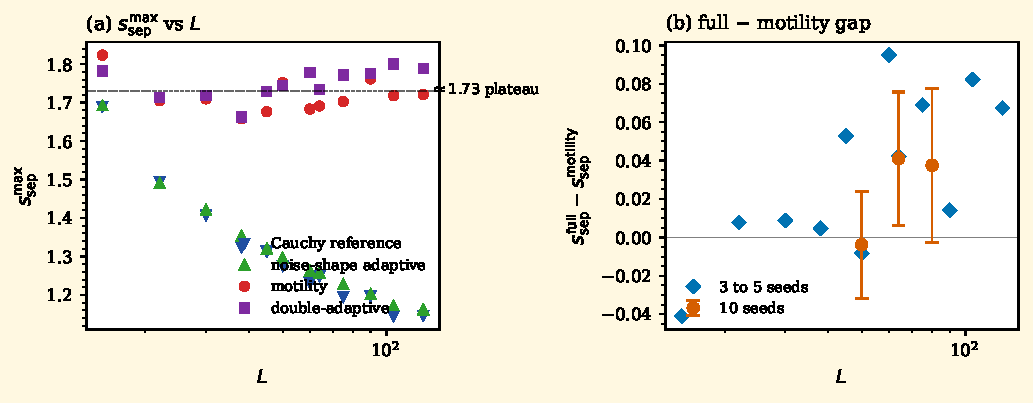
\includegraphics[width=0.92\linewidth]{fig_double_Lfine_gap.pdf}
    \caption{Twelve-size $s_{\rm sep}$ scan: seven-size FSS (three
    seeds) plus five intermediate sizes $L \in \{38, 50, 60, 75,
    105\}$ (five seeds). (a) $s_{\rm sep}^{\max}$ vs $L$ for
    motility-only and double-adaptive; (b) their gap.}
    \label{fig:Lfine_gap}
\end{figure}

The gap is small at the two smaller fine-grid sizes ($\le
|0.01|$ at $L = 38, 50$) and turns positive in $[+0.07, +0.10]$
across $L = 60$ to $105$, the small-$L$ closure following the
mode-dependent location of the $s_{\rm sep}$ peak in $\eta$. A
ten-seed paired gap at the full-mode $\chi$-peak $\eta$
(Table~\ref{tab:gap_se}) tells much the same story: $+0.165$ ($95\%$
seed-bootstrap CI $[+0.109, +0.223]$, Wilcoxon $p = 0.002$) at
$L = 64$, but within noise of zero at $L = 50, 80$ ($p \ge
0.56$), so only $L = 64$ is robustly positive.

\begin{table}[h]
\centering
\caption{Paired $s_{\rm sep}$ gap between double-adaptive
and motility-only at the full-mode $\chi$-peak $\eta$, ten
seeds per cell. As $s_{\rm sep}$ is a ratio of extreme order
statistics with heavy tails, we judge the gap with a $95\%$
paired seed-bootstrap CI ($B = 10\,000$) and a Wilcoxon
signed-rank $p$ rather than a Gaussian $z$.}
\label{tab:gap_se}
\small
\begin{tabular}{l c c c}
\toprule
$L$ & gap (full $-$ motility) & $95\%$ bootstrap CI & Wilcoxon $p$ \\
\midrule
$50$ & $+0.020$ & $[-0.038, +0.080]$ & $0.70$ \\
$64$ & $+0.165$ & $[+0.109, +0.223]$ & $0.002$ \\
$80$ & $+0.024$ & $[-0.035, +0.081]$ & $0.56$ \\
\bottomrule
\end{tabular}
\end{table}

The $s_{\rm sep}$ advantage is therefore real and significant at
$L \simeq 64$ but small and seed-budget-limited at neighbouring
sizes. Like the susceptibility excess, it is the noise-shape
channel reading out at each mode's own noise, the same dense-phase
rectification rather than an independent cooperation.

\subsection*{Cluster-size distribution and number fluctuations}
\label{sec:supp-clusters}

Where $s_{\rm sep}$ reports a single contrast ratio, the
cluster-size distribution reports the whole dense-phase
morphology: a homogeneous fluid carries small fluctuations, a
spinodal regime a power-law tail with 2D exponent near $-2$, a
binodal regime one giant cluster coexisting with small ones. We
coarse-grain on a
$10 \times 10$ grid, threshold each cell at $1.5$ times the median
occupancy, and run periodic-aware connected-component labelling on
the binary mask; a grid-free DBSCAN check ($\varepsilon = R_a$,
four-point core) ranks the modes the same way (ten seeds,
$L = 30$).

\begin{figure}[htbp]
    \centering
    
\includegraphics[width=\linewidth]{fig_double_cluster_summary.pdf}
    \caption{Dense-phase structure across the four modes at
    $L = 30$, ten seeds. (a)--(c) seed-averaged cluster count, max
    size and mean size ($\pm 1$ SE): double-adaptive concentrates
    the dense mass into a few large droplets
    ($\langle s_{\max}\rangle = 177$ vs $55$). (d) number
    fluctuations $\mathrm{Var}(N_{\rm box})$ vs
    $\langle N_{\rm box}\rangle$ with fitted $\zeta$ (dashed Poisson
    reference). (e) cluster-size distribution $P(s)$, hue keying the
    mode and line style the noise $\eta \in \{0.02, 0.05, 0.10,
    0.20\}$.}
    \label{fig:cluster_summary}
\end{figure}

\begin{figure}[htbp]
    \centering
    
\includegraphics[width=0.95\linewidth]{fig_double_cluster_map.pdf}
    \caption{Real-space cluster identification at near-critical
    $\eta$, single seed, motility-only (top) and double-adaptive
    (bottom) across $L \in \{30, 90, 128\}$ (panels (a)--(f)).
    Dense-bin particles ($> 1.5\times$ median occupancy on a
    $10 \times 10$ grid) are arrows coloured by connected-component
    cluster; dilute-bin particles grey; dense bins ochre-shaded;
    zoom inset per panel.}
    \label{fig:cluster_map}
\end{figure}

The Cauchy and noise-shape modes give only marginal density
fluctuations (a few clusters per seed, max size near the threshold
floor). Both motility-active modes fragment the box into $\sim
160$--$190$ dense clusters, but the full mode pushes the largest
one far higher (max size $176.6 \pm 42.3$ against $55.0 \pm 7.5$
for motility-only). Because the dense-phase estimators are
heavy-tailed, we report each full-minus-motility gap with its
$95\%$ seed-bootstrap CI ($B = 10\,000$) and a Wilcoxon
signed-rank test rather than a Gaussian $z$. The two modes differ
on cluster count by $-25.9$ ($[-62.9, +19.5]$, $p = 0.19$; not
significant) and on max size by $+121.6$ ($[+40.5, +206.6]$,
$p = 0.02$), so max size is the diagnostic that carries the
signal and the count is not. The rectification fuses dense patches
into a few large clusters at conserved total dense area
(Fig.~\ref{fig:cluster_map}).

The dense-phase distribution $P(s)$ sharpens the same reading
(Fig.~\ref{fig:cluster_summary}e). The two fixed-speed references
never grow a dense-phase tail (giant-cluster fraction at the
binning floor, $\langle s_{\max}/N\rangle \simeq 0.001$--$0.002$,
the Vicsek band instability at $\rho_0 = 2.22$ too weak to
nucleate a dense phase with the motility channel off), while both
motility-active modes carry one. At their near-critical operating
points the double-adaptive tail is steeper ($\tau = 2.01$ against
$1.74$) with a $2.6$-fold larger giant-cluster fraction ($0.018$
versus $0.007$), the binodal signature of mass concentrated into a
few large droplets.

A phase-separated active fluid leaves a second, independent trace
in its density fluctuations. We measure the variance of the
particle number $N_{\rm box}$ in nested square sub-boxes against
its mean,
$\mathrm{Var}(N_{\rm box}) \sim \langle N_{\rm box}\rangle^{2\zeta}$,
at $L = 30$, near-critical $\eta$ and ten seeds
(Fig.~\ref{fig:cluster_summary}d); a homogeneous fluid sits at the
Poisson value $\zeta = 1/2$, a polar flock at the Toner--Tu
value $\zeta \simeq 0.8$ \citep{TonerTu1995}. The two
fixed-noise-shape references stay Poissonian ($\zeta = 0.57$
Cauchy, $0.58$ noise-shape), while the two motility-active modes
fluctuate anomalously, $\zeta = 0.79$ (motility-only) and $0.82$
(double-adaptive), both straddling the polar-flock prediction. The
diagnostic therefore confirms phase separation in the
motility-active modes but does not separate them from each other,
which is why the main text reads the rectification off the
dense-quartile observables instead.

\subsection*{Density-conditioned transport}
\label{sec:supp-msd}

A heading that stays correlated for longer should carry the
particle further, so we turn the persistence result of the main
text into transport with the mean squared displacement
$\langle\Delta r^2\rangle(\tau)$, conditioned on the density class
at the time origin and unwrapped across the periodic box
(Fig.~\ref{fig:dynamics}d). The dense phase is ballistic, a
coherent comoving ordered droplet, with exponent
$\gamma_{\rm dense} = 2.01 \pm 0.01$ for the double-adaptive model
and $1.93$ for motility-only, while the dilute gas is
super-diffusive but sub-ballistic, $\gamma_{\rm dilute} = 1.59$
and $1.45$, the fast free particles losing direction to their
heavy-tailed turning. The two fixed-speed references stay
near-diffusive ($\gamma \simeq 1.0$--$1.1$ in both quartiles):
building no dense phase, their fast but heavy-tailed motion simply
randomises. The double feedback raises the exponent in both phases
and lifts the dense-phase displacement at $\tau = 2\,000$ steps by
$66\%$ ($235.7$ against $142.2$ in box units), so the Gaussian
gate makes the dense droplets advance as cleaner ballistic units.

\bibliographystyle{plainnat}
\bibliography{refs}

\end{document}
